\setlength{\parskip}{\baselineskip}
\section*{Teoría de Ciclos}

%- - - - - - - - - - - - - - - - - Título - - - - - - - - - - - - - - - - - -%
\begin{frame}[c] 
\centering
\huge \textbf{Teoría de ciclos}
\end{frame}

% - - - - - - - - - - - - - - - - - - - - - Slide 01 - - - - - - - - - - - - - - - - - - - - - - -
\begin{frame}{Teoría de Ciclos}
    \begin{center}\textbf{Definición}\end{center}
    \justify
    \hspace{5mm}
    Un bucle (ciclo o lazo, loop en inglés) es cualquier construcción de programa que
    repite una sentencia o secuencia de sentencias un número de veces. La sentencia (o
    grupo de sentencias) que se repiten en un bloque se denomina cuerpo del bucle y
    cada repetición del cuerpo del bucle se llama iteración del bucle.
\end{frame}


% - - - - - - - - - - - - - - - - - - - - - Slide 02 - - - - - - - - - - - - - - - - - - - - - - -
\begin{frame}{Teoría de Ciclos}
    \begin{center}\textbf{Contadores}\end{center}
    \vspace{-2mm}
    Es una variable cuyo valor se incrementa o decrementa en una cantidad constante cada vez que se produce un determinado suceso o acción en cada repetición; dicha variable controla o determina la cantidad de veces que se repite un proceso o dato.
    \begin{block}{Contadores}
        int contador 5 1; //variable con valor inicial de 1\\
        contador++; o ++contador; o contador+=1;
    \end{block}
\end{frame}


% - - - - - - - - - - - - - - - - - - - - - Slide 03 - - - - - - - - - - - - - - - - - - - - - - -
\begin{frame}{Teoría de Ciclos}
    \vspace{-1mm}
    \begin{center}\textbf{Acumuladores}\end{center}
    \vspace{-3mm}
    Un acumulador realiza la misma función que un contador con la diferencia de que el incremento o decremento es variable. Es una variable que acumula sobre sí misma un conjunto de valores, para tener la acumulación de todos ellos en una sola variable. Almacena cantidades resultantes de operaciones sucesivas.
    \begin{block}{Acumuladores}
        int acumulador 50;\\
        acumulador = acumulador + valor;
    \end{block}
\end{frame}


% - - - - - - - - - - - - - - - - - - - - - Slide 04 - - - - - - - - - - - - - - - - - - - - - - -
\begin{frame}{Teoría de Ciclos}
    \begin{center}\textbf{Centinela}\end{center}
    \hspace{5mm}
    El centinela es una variable que inicia con un valor, luego dentro de un bucle este valor cambia, haciendo falsa la condición del ciclo y por lo tanto indicará el fin del ciclo (el usuario puede determinar cuándo hacerlo). La repetición controlada por centinela se considera como una repetición indefinida (se desconoce el número de repeticiones).
\end{frame}



% - - - - - - - - - - - - - - - - - - - - - Slide 05 - - - - - - - - - - - - - - - - - - - - - - -
\begin{frame}{Teoría de ciclos}

    \begin{center}\textbf{Ciclo While}\end{center}
    \hspace{5mm}
    Un ciclo \textbf{while} tiene una condición (expresión lógica) que controla la secuencia de repetición. La posición de esta condición es previo al cuerpo del ciclo, de modo que, cuando se ejecuta, se evalúa la condición antes de que se ejecute el cuerpo del bucle.
\end{frame}


% - - - - - - - - - - - - - - - - - - - - - Slide 06 - - - - - - - - - - - - - - - - - - - - - - -
\begin{frame}[fragile]{Tipos de Ciclos}
\begin{center}\textbf{Sintaxis}\end{center}
\begin{columns}[t]
    \begin{column}{0.4 \textwidth}
        \begin{lstlisting}
while(condicion)
    sentencia;
\end{lstlisting}
    \end{column}
    \begin{column}{0.4 \textwidth}
        \begin{lstlisting}
while(condicion)
{
    senctencia_1;
    .
    .
    sentencia_n;
}
\end{lstlisting}
    \end{column}
\end{columns}
\end{frame}


% - - - - - - - - - - - - - - - - - - - - - Slide 07 - - - - - - - - - - - - - - - - - - - - - - -
\begin{frame}[t]{Teoría de ciclos}
    \vspace{-5mm}
    \begin{center}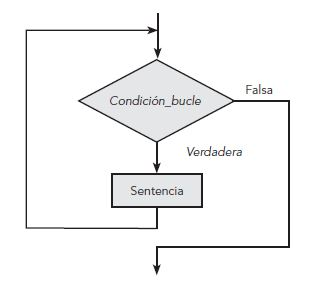
\includegraphics[scale=0.4]{flujoWhile.JPG}\vspace{-5mm}\end{center}
    \justify
    \hspace{5mm}
    El diagrama indica que la ejecución de la sentencia se repite mientras la condición permanece verdadera y termina cuando se hace falsa. También que la condición del ciclo se evalúa antes de ejecutar el cuerpo del ciclo, si esta condición es inicialmente falsa, el cuerpo del ciclo no se ejecutará. En otras palabras, el cuerpo de un bucle while se ejecutará cero o más veces.
\end{frame}



% - - - - - - - - - - - - - - - - - - - - - Slide 08 - - - - - - - - - - - - - - - - - - - - - - -
\begin{frame}[fragile]{Teoría de ciclos}
\begin{center}
    \textbf{CICLO DE MUESTRA CON \textit{WHILE}}
\end{center}
\lstinputlisting[style=customc]{codigos/ciclos/cicloMuestra.c}
\end{frame}



% - - - - - - - - - - - - - - - - - - - - - Slide 09 - - - - - - - - - - - - - - - - - - - - - - -
\begin{frame}[fragile]{Teoría de ciclos}
    \begin{center}
        \textbf{Ciclo Infinito}
    \end{center}
    \justify
    Si la variable de control no se actualiza el ciclo se ejecutará “siempre” (ciclo infinito). Un ciclo infinito (sin terminación) se produce cuando la condición del permanece y no se hace falsa en ninguna iteración.
    \vspace{-2mm}
\begin{center}
    \begin{tabular}{c}
            \begin{lstlisting}
/* bucle infinito */
contador = 1;
while (contador < 100)
{
    printf("%d \n", contador);
    contador--;
}
\end{lstlisting}
    \end{tabular}
\end{center}
\end{frame}


% ***********************************************************************************************
% *                                     TIPOS DE CICLOS                                         *
% ***********************************************************************************************
% - - - - - - - - - - - - - - - - - - - - - Slide 10 - - - - - - - - - - - - - - - - - - - - - - -
\begin{frame}{Tipos de ciclos}
\begin{center}
    \textbf{Ciclos controlados por contador}
\end{center}
\justify
\hspace{5mm}
La repectición controlada por un contador se utiliza cuando se conoce el número de repeticiones antes de que un ciclo empiece a ejecutarse; es decir, cuando hay una repetición definida.
\end{frame}

% - - - - - - - - - - - - - - - - - - - - - Slide 11 - - - - - - - - - - - - - - - - - - - - - - -
\begin{frame}{Tipos de ciclos}
\begin{center}
    \textbf{Ciclos controlados por centinela}
    \justify
    \hspace{5mm}
    La repetición controlada por un centinela se utiliza cuando no se conoce el número de repeticiones antes de que un ciclo empiece a ejecutarse; es decir, cuando hay una repetición indefinida.
\end{center}
\end{frame}


% - - - - - - - - - - - - - - - - - - - - - Slide 12 - - - - - - - - - - - - - - - - - - - - - - -
\begin{frame}[fragile,t]{Tipos de ciclos}
    \begin{center}\textbf{Ejemplos}\end{center}
    \begin{columns}[t]
        \begin{column}{0.57 \textwidth}
            \begin{block}{Por contador}
                El siguiente ciclo cuenta hasta 10
                \begin{lstlisting}
int x = 0;
while( x < 10 )
    printf("X: %d\n", x++);
\end{lstlisting}
            \end{block}
        \end{column}
        \begin{column}{0.5 \textwidth}
            \begin{block}{Por centinela}
                Visualizar n asteriscos
                \begin{lstlisting}
contador = 0;
while( contador < n )
{
    printf(" * ");
    contador++;
}/*Fin del while*/
\end{lstlisting}
            \end{block}
        \end{column}
    \end{columns}
\end{frame}

%***************************************************************************
%*                               CICLO FOR                                 *
%***************************************************************************

% - - - - - - - - - - - - - - - - - - - - - Slide 13 - - - - - - - - - - - - - - - - - - - - - - -
\begin{frame}{Tipos de ciclos}{Ciclo For}
\begin{center}
    \textbf{Ciclo For}
\end{center}
La sentencia \textbf{for} es un método para ejecutar un bloque de sentencias un número fijo de veces. El \textit{ciclo \textbf{for}} se diferencia del \textit{ciclo \textbf{while}} en que las operaciones de control del ciclo se sitúan en un solo sitio: la cabecera de la sentencia.
\end{frame}

% - - - - - - - - - - - - - - - - - - - - - Slide 14 - - - - - - - - - - - - - - - - - - - - - - -
\begin{frame}[fragile, t]{Tipos de ciclos}
    \begin{center}
        \textbf{Sintaxis}
    \end{center}
    \vspace{-5mm}
    \begin{lstlisting}[basicstyle=\ttfamily\small]
for(Inicialización; CondiciónIteración;Incremento)
    sentencias
\end{lstlisting}
    \vspace{-3mm}
{\small \begin{itemize}
    \item \textcolor{blue}{Inicialización:} Inicializa la variable de control del ciclo.\pause
    \item \textcolor{blue}{CondicióIteración:} Expesión lógica que determina se las sentencias se han de ejecutar (mientras sea verdadera)\pause
    \item \textcolor{blue}{Incremento:} Incrementa o decrementa la variable de control de bucle.\pause
    \item \textcolor{blue}{sentencias:} Sentencias a ejecutar en cada iteración del bucle
\end{itemize}}
\end{frame}


% - - - - - - - - - - - - - - - - - - - - - Slide 15 - - - - - - - - - - - - - - - - - - - - - - -
\begin{frame}{Tipos de ciclos}
    \centering
    \textbf{Diagrama de Flujo del ciclo \textit{For}}\\
    \vspace{3mm}
    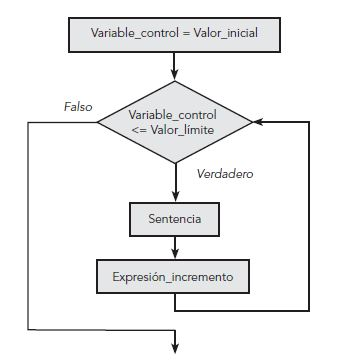
\includegraphics[scale=0.6]{flujoFor.jpg}
\end{frame}



% - - - - - - - - - - - - - - - - - - - - - Slide 16 - - - - - - - - - - - - - - - - - - - - - - -
\begin{frame}[fragile]{Tipos de ciclos}
    \centering
    \textbf{Ejemplo}
    \lstinputlisting[style=customc]{codigos/ciclos/cicloFor.c}
\end{frame}

\begin{frame}{Tipos de ciclos}
    \begin{center}\textbf{Ciclo do-while}\end{center}
    \justify
    La sentencia \textbf{\textit{do-while}} se utiliza para especificar un bucle condicional que se ejecuta al menos una vez. Esta situación se suele dar en algunas circunstancias en las que se ha de tener la seguridad de que una determinada acción se ejecutará una o varias veces, pero al menos una vez.
\end{frame}

% - - - - - - - - - - - - - - - - - - - - - Slide 17 - - - - - - - - - - - - - - - - - - - - - - -
\begin{frame}[fragile]{Tipos de ciclos}
    \begin{center}\textbf{SIntaxis}\end{center}
    \begin{columns}
        \begin{column}{0.5 \textwidth}
            \begin{lstlisting}
do
    sentencia
while(expresion);
            \end{lstlisting}
        \end{column}
        \begin{column}{0.5 \textwidth}
            \begin{lstlisting}
do
{
    sentencias;
}while(expresion);
            \end{lstlisting}
        \end{column}
    \end{columns}
\end{frame}

% - - - - - - - - - - - - - - - - - - - - - Slide 17 - - - - - - - - - - - - - - - - - - - - - - -
\begin{frame}{Tipos de ciclos}
    \begin{center}\textbf{Sintaxis}\end{center}
    \begin{columns}
        \begin{column}{0.5 \textwidth}
                \hspace{2mm}
                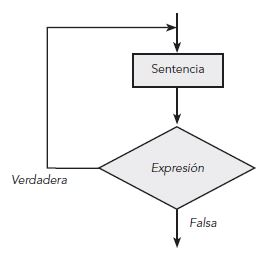
\includegraphics[scale=0.7]{flujoDoWhile.jpg}
        \end{column}
        \begin{column}{0.5 \textwidth}
            \justify
            Después de cada ejecución de sentencia se evalúa expresión: si es falsa, se termina el
            ciclo y se ejecuta la siguiente sentencia; si es verdadera, se repite el cuerpo del ciclo (la sentencia).
        \end{column}
    \end{columns}
\end{frame}

\begin{frame}[fragile]{Tipos de ciclos}
    \begin{center}\textbf{Ejemplo}\end{center}
    \lstinputlisting[style=customc]{codigos/ciclos/cicloDoWhile.c}
\end{frame}